%=== Préambule ===========================================================

\documentclass{beamer}
\usepackage{pdfpages}
\usepackage{braille}
%\usepackage[english]{babel}
%\usepackage[latin1]{inputenc}
%\usepackage[cyr]{aeguill}
\usepackage[english]{babel}
\usepackage{xspace}
\usepackage{pifont}
\usepackage{hyperref}
\usepackage{listings}
\usepackage{csquotes}
\usepackage{graphicx}
\usepackage{animate,media9} %,movie15}
\usepackage{wrapfig}
\usepackage{pdfpages}
\usepackage{tikz}
\usepackage{natbib}
\uselanguage{English}
\usepackage{fontawesome5}
\languagepath{English}
\setcounter{tocdepth}{1}
\usepackage{setspace}
\usepackage{amsmath}
\def\glasses{{\sffamily 
\leavevmode\rlap{%
\rotatebox[origin=tr]{125}{J}\kern1ex%  
\rotatebox[origin=tr]{125}{J}}% 
\rotatebox[origin=c]{-90}{D}%   
\rotatebox[origin=c]{-90}{D}}%
\def\ialy{\sffamily 
\resizebox{1ex}{1.5ex}{\reflectbox{\rotatebox[origin=]{75}{J}}}\kern-1pt%
\rlap{\tiny$\ ^\bullet\kern2.5pt^\bullet$ }%
\rotatebox[origin=c]{-90}{D}%   
\rotatebox[origin=c]{-90}{D}\kern-1pt%  
\resizebox{1ex}{1.5ex}{\rotatebox[origin=]{75}{J}}}}


\lstset{
  numbers=left,
  basicstyle=\tiny\ttfamily,      
  breaklines=true, 
  showtabs=false,
  showstringspaces=false,
}  

%=== Configuration de Beamer et du thème metropolis ======================
\usepackage{bbding}
\usetheme[background=light]{metropolis}
\usepackage[clock]{ifsym}

\definecolor{mLightBrown}{HTML}{000000}
\definecolor{black}{HTML}{000000}
\setbeamercolor{structure}{fg=black,bg=mLightBrown}
\setbeamercolor{palette primary}{%
	use=normal text,
	fg=normal text.bg,
	bg=mLightBrown
}
%\setsansfont[BoldFont={Linux Libertine G Bold},Numbers={OldStyle}]{Linux Libertine G}

\metroset{block=fill}

%=== Page de titre =======================================================

%path to logo and biblio -> to be adapted to your local directories 
\newcommand\dirlogo{../../logos/}
\newcommand\dirbiblio{../../biblio}



\title{{\normalsize \vskip 1.5cm {\bf Ongoing work about the 2023 Mw7.8 Turkey Earthquake}}}
\author{ {\bf Hugo Sánchez-Reyes and Emmanuel Caballero-Leyva}  
\\ 
\\
\\
\vfill
{ISTerre} \\
\textit{Seminaire}
%\hskip 2cm a
}

\date[2022]{\today}

\subject{}

\titlegraphic{\centering \vspace{-18pt}
\includegraphics[height=1.2cm]{../../logos/logo_seminar_2022.pdf} \par \vskip 5 cm \hskip 3 cm \braille{IRD} } %\qquad  
\includegraphics[height=1.4cm]{../../logos/anr_eqtime.png} \par }


\addtobeamertemplate{frametitle}{}{%
\begin{tikzpicture}[remember picture,overlay]
  \node[anchor=north east,yshift=0.0ex] at (current page.north east) {
\includegraphics[height=4ex]{../../logos/IRD_neg.png}};
  %\node[anchor=north east,yshift=0.5ex] at (current page.north east) {\includegraphics[height=3.3ex]{\dirlogo/seiscope_color_light_background}};
\end{tikzpicture}}



%=== Document ============================================================

\begin{document}

% --- Préambule ---------------------------------------------------------------

\begin{frame}
    \titlepage
\end{frame}

\section{Emmanuel's work: \\ Detecting other events (foreshocks)}

\begin{frame}
 {Work by Emmanuel Caballero-Leyva (Waves Team)}
 
 \begin{minipage}{1\linewidth}
 \vskip -0.2cm \hskip -0.5cm 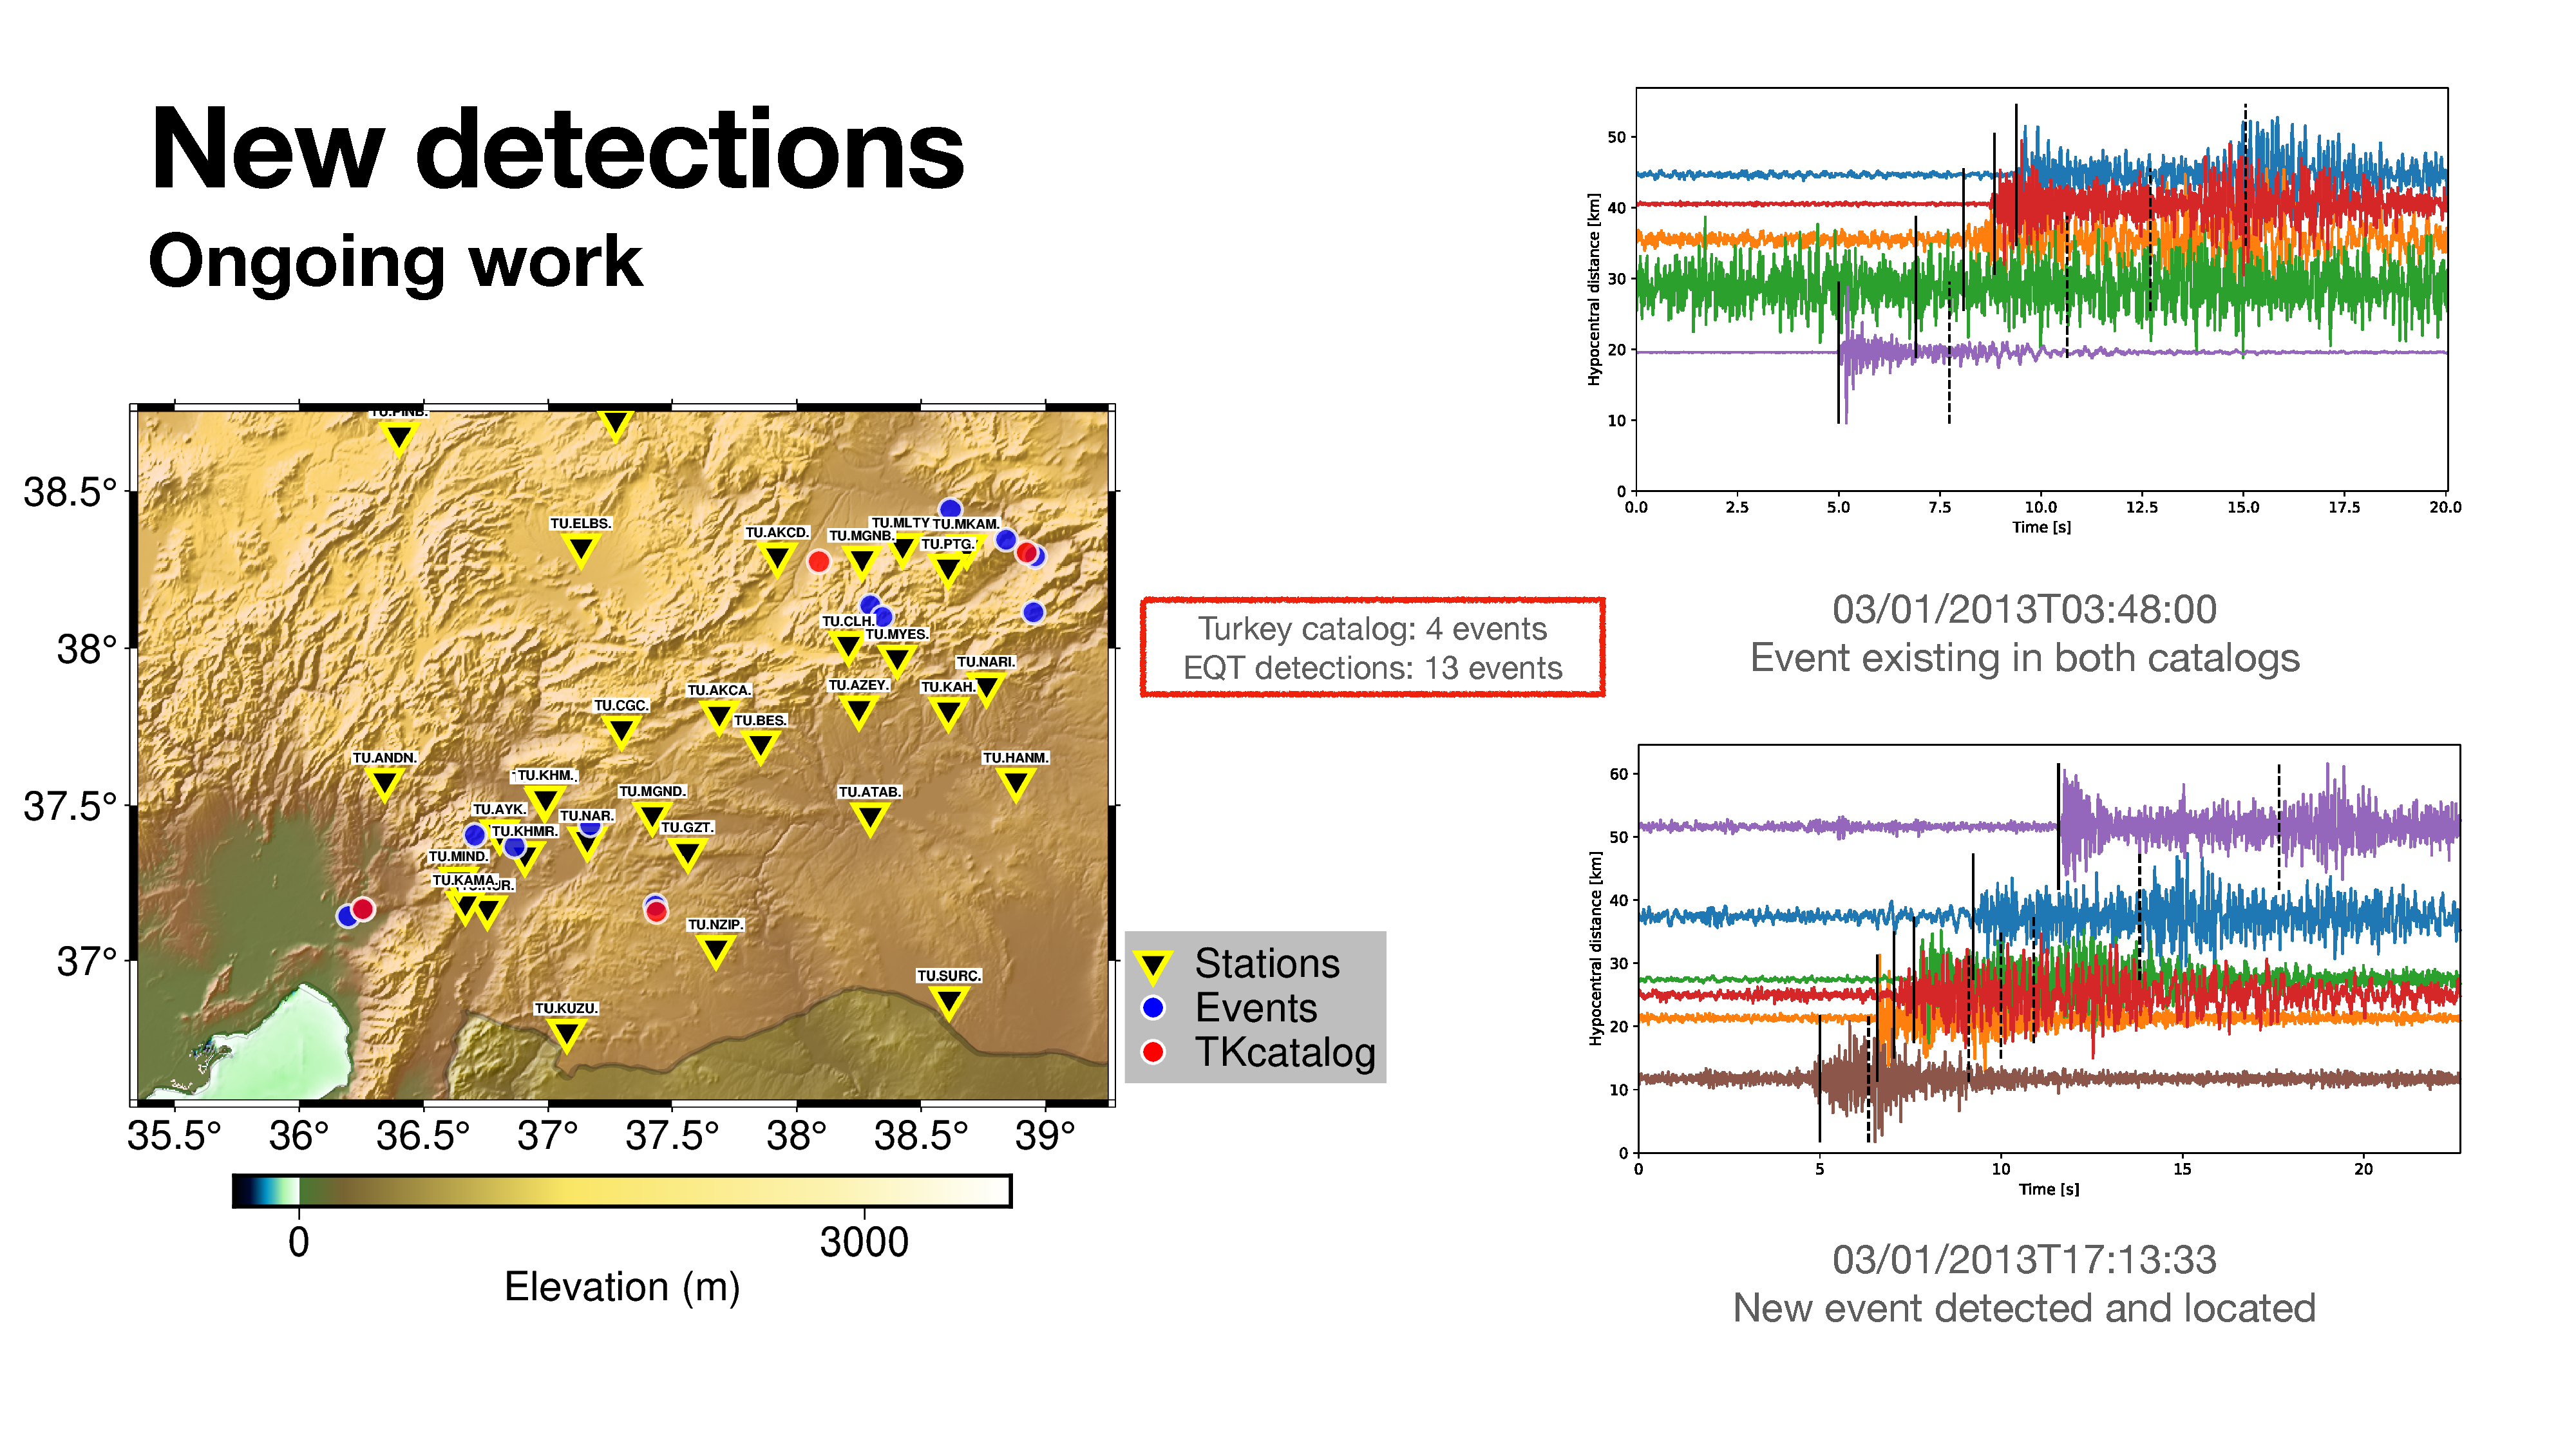
\includegraphics[width=1.1\linewidth]{images/presentation_TK.pdf} \\
 \end{minipage}

 \vskip -0.5cm
 {\hfill \scriptsize using EQTransformer 
 from SeisBench \\ \hfill \citep{SeisBench} ... thanks Jannes!}

\end{frame}


\begin{frame}
 {Work by Hugo: Slip inversion? ... ongoing work}
 
 \vskip -1cm \begin{minipage}{0.51\linewidth}
  \hskip -2.8cm
  \animategraphics[autoplay,loop,width=1.7\textwidth]{1}{images/video/fig_}{01}{09} %27 
\end{minipage} 
\begin{minipage}{0.47\linewidth}
\vskip 1cm Why did it start like this? \\ and why there? :
\vskip 0.1cm
\begin{itemize}
 \item Stress field?
 \item Geometry?
 \item A mixture?
\end{itemize} %\\ \vskip 0.1cm
\vskip 0.2cm 
\centering
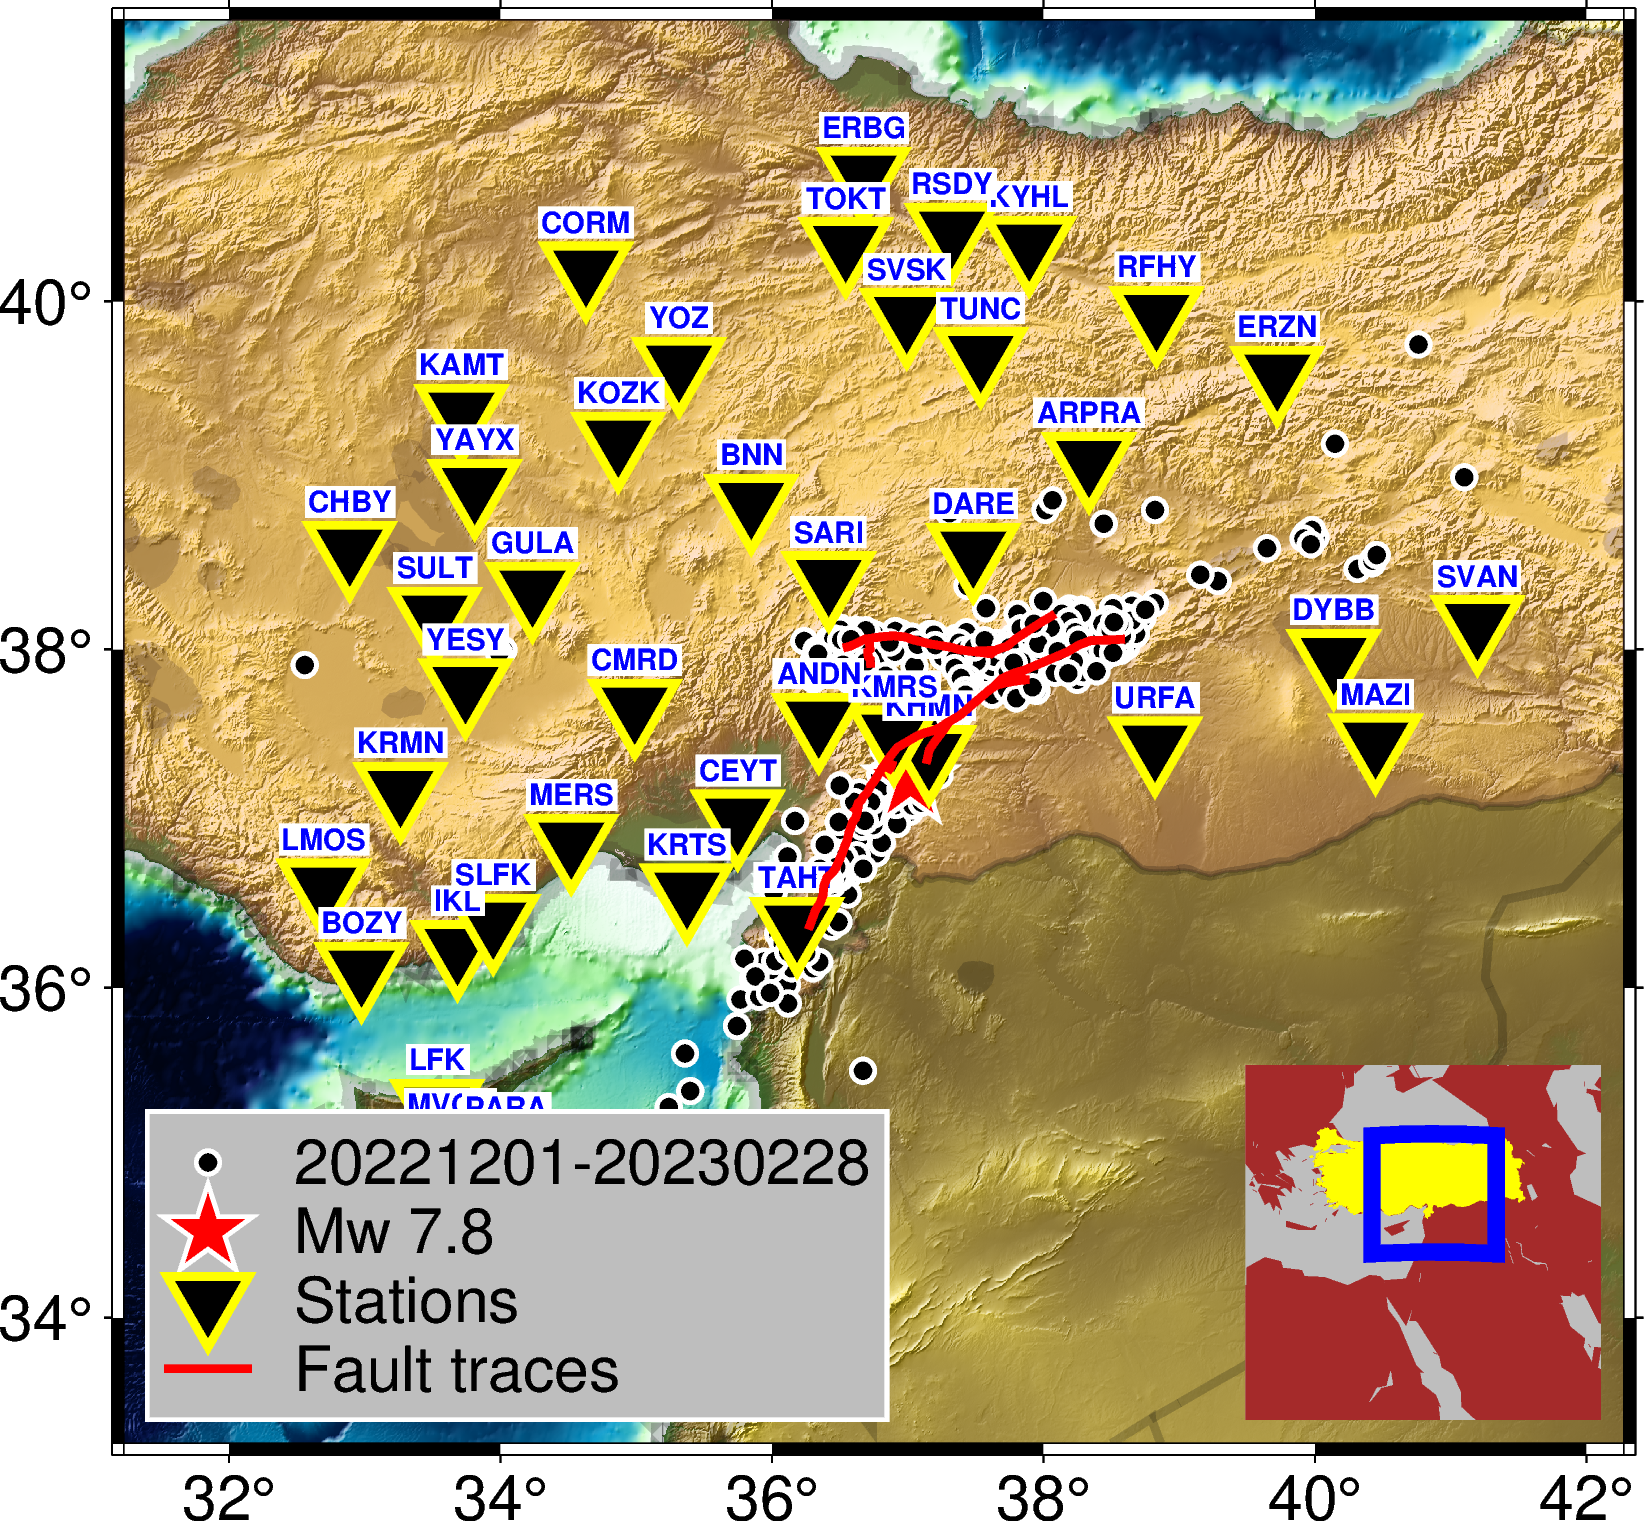
\includegraphics[width=1\linewidth]{images/Map.png}

\end{minipage} 
 
\end{frame}


\begin{frame}
 {Work by Hugo: Slip inversion? ... ongoing work}
 
 \vskip -0.5cm \begin{minipage}{0.51\linewidth}
  \hskip -0.8cm
  \animategraphics[autoplay,loop,width=1.2\textwidth]{4}{images/video/figa_}{01}{01} %27 
\end{minipage} 
\begin{minipage}{0.47\linewidth}
\vskip 0.7cm Why did it start like this? \\ and why there? :
\vskip 0.1cm
\begin{itemize}
 \item Stress field?
 \item Geometry?
 \item A mixture?
\end{itemize}
\end{minipage} \\ \vskip 0.2cm \pause
\begin{minipage}{0.45\linewidth}
 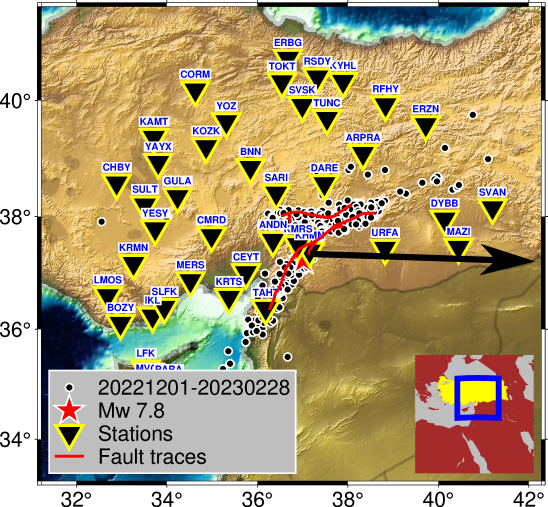
\includegraphics[width=1\linewidth]{images/Map2.png}
\end{minipage}
\begin{minipage}{0.45\linewidth}
 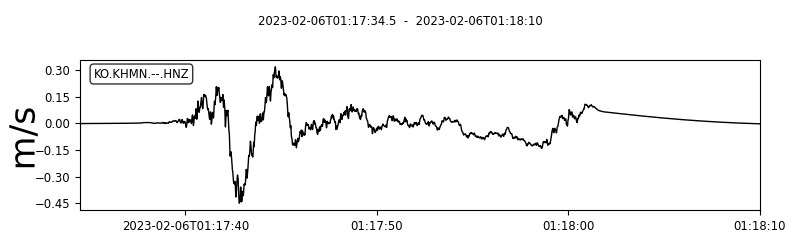
\includegraphics[width=1.4\linewidth]{images/p1.png}
\end{minipage}
 
\end{frame}


\begin{frame}
 {Work by Hugo: Slip inversion? ... ongoing work}
 
 \vskip -0.5cm \begin{minipage}{0.51\linewidth}
  \hskip -0.8cm
  \animategraphics[autoplay,loop,width=1.2\textwidth]{4}{images/video/figa_}{01}{01} %27 
\end{minipage} 
\begin{minipage}{0.47\linewidth}
\vskip 0.7cm Why did it start like this? \\ and why there? :
\vskip 0.1cm
\begin{itemize}
 \item Stress field?
 \item Geometry?
 \item A mixture?
\end{itemize}
\end{minipage} \\ \vskip 0.2cm 
\begin{minipage}{0.45\linewidth}
 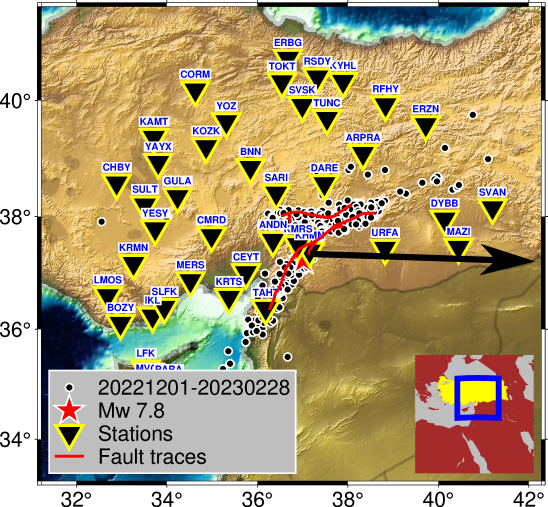
\includegraphics[width=1\linewidth]{images/Map2.png}
\end{minipage}
\begin{minipage}{0.45\linewidth}
 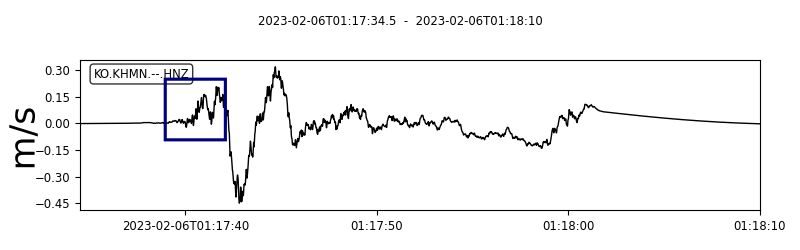
\includegraphics[width=1.4\linewidth]{images/p1z.png}
\end{minipage}
 
\end{frame}


\begin{frame}
 {Work by Hugo: Slip inversion? ... ongoing work}
 
 \vskip -0.5cm \begin{minipage}{0.51\linewidth}
  \hskip -0.8cm
  \animategraphics[autoplay,loop,width=1.2\textwidth]{4}{images/video/figa_}{01}{01} %27 
\end{minipage} 
\begin{minipage}{0.47\linewidth}
\vskip 0.7cm Why did it start like this? \\ and why there? :
\vskip 0.1cm
\begin{itemize}
 \item Stress field?
 \item Geometry?
 \item A mixture?
\end{itemize}
\end{minipage} \\ \vskip 0.2cm 
\begin{minipage}{0.45\linewidth}
 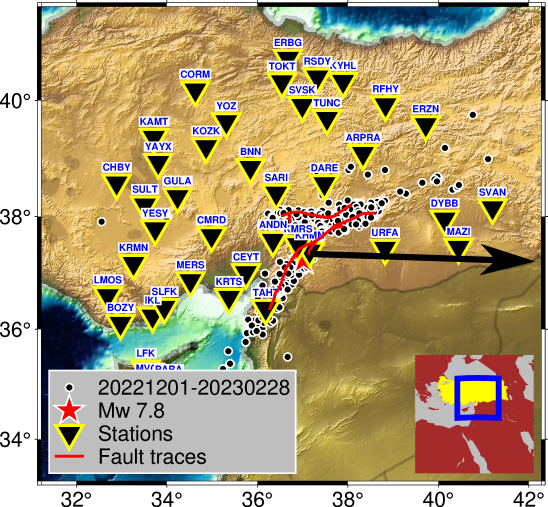
\includegraphics[width=1\linewidth]{images/Map2.png}
\end{minipage}
\begin{minipage}{0.45\linewidth}
 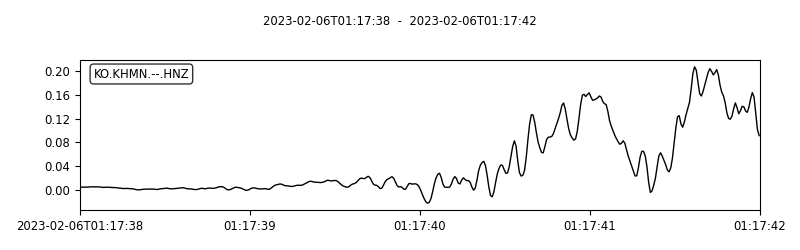
\includegraphics[width=1.4\linewidth]{images/p2.png}
 \centering I will focus on this initial phase!
\end{minipage}
 
\end{frame}




\begin{frame}
 {First estimation of traveltimes: ???}
 
 \begin{center}
 \vskip -0.5cm 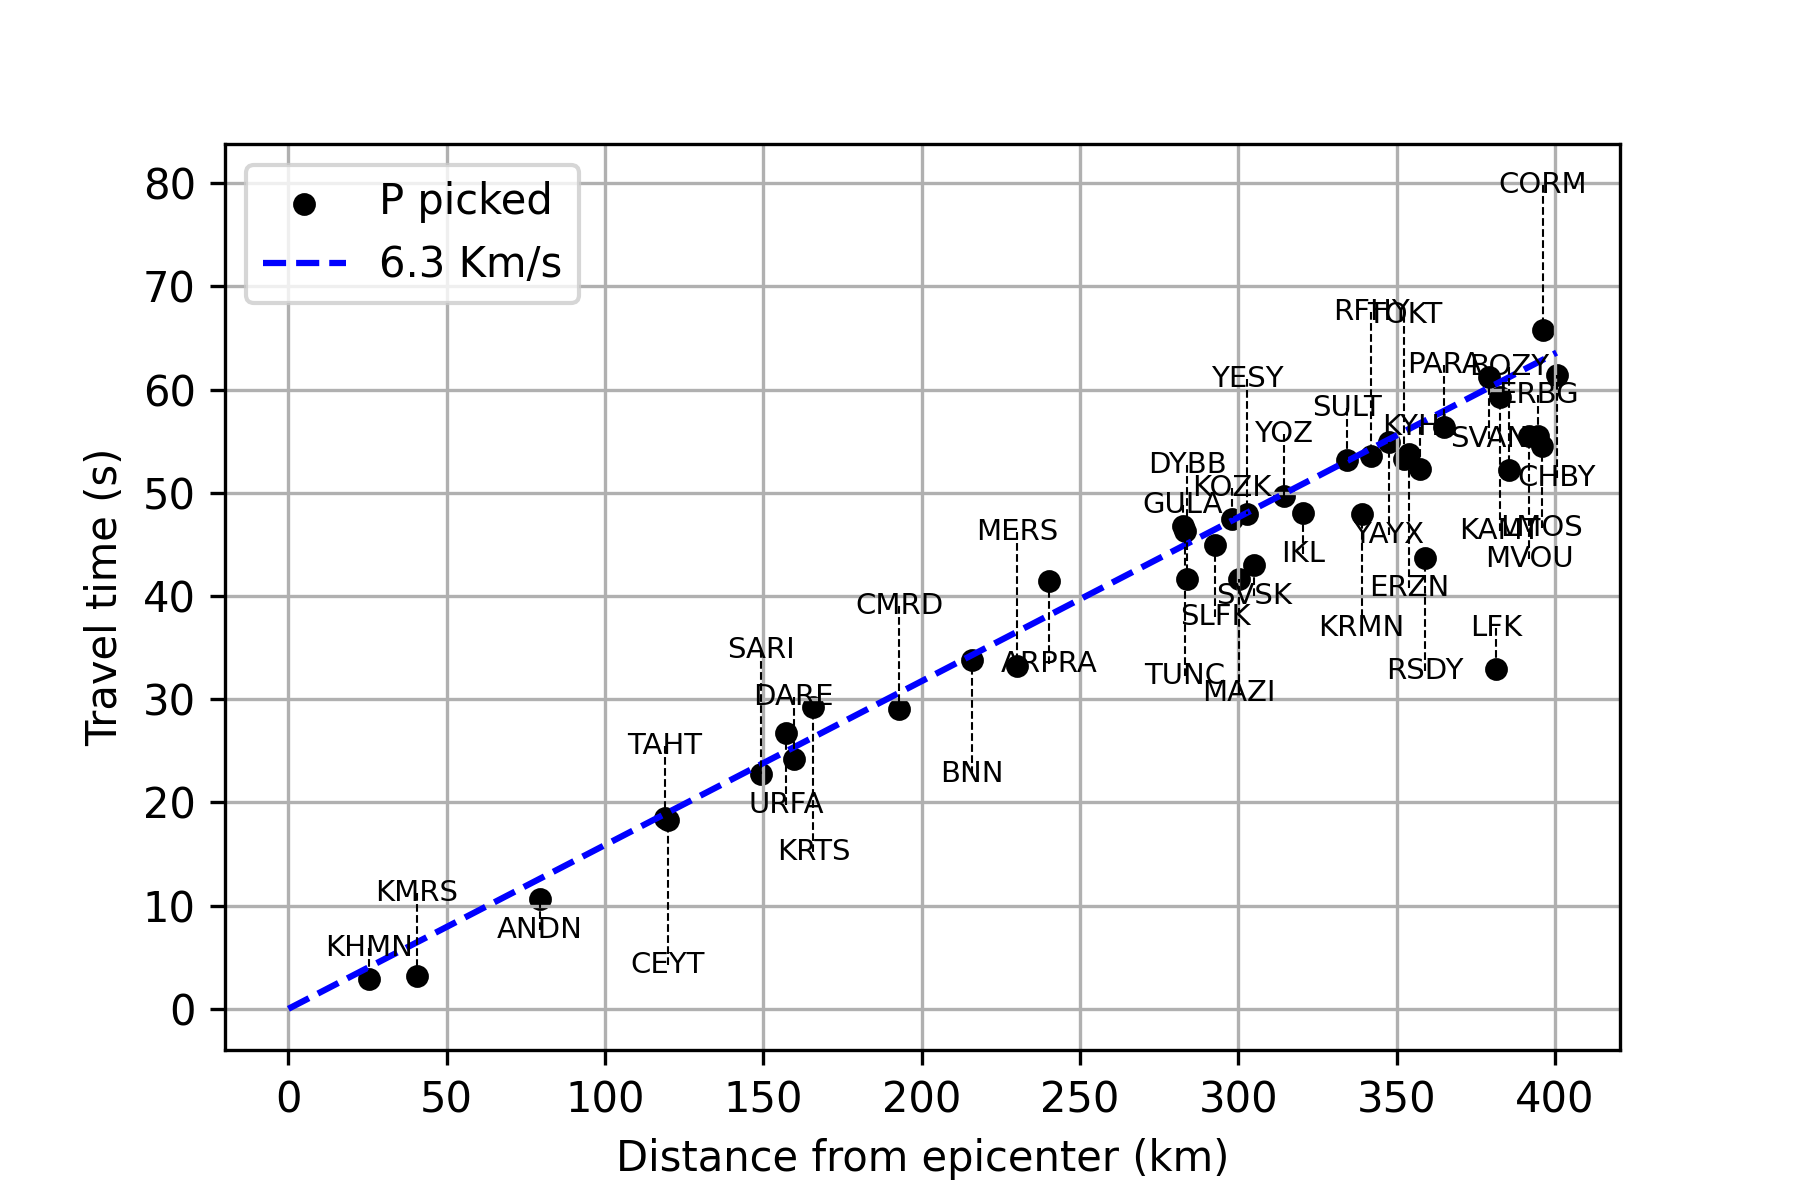
\includegraphics[width=0.9\linewidth]{images/tt_p.png}  
 \end{center}

 \vskip -0.5cm
 {\scriptsize
 Hypocenter: ??? \\
 {\bf Orfeus: longitude = 37.08 E, latitude = 37.17 N, depth = 20 km} \\ 
 GCMT: longitude = 37.021 E, latitude = 37.225 N, depth = 10 km \\
 USGS: longitude = 37.019 E, latitude = 37.220 N, depth = 10 km \\
 AFAD: Longitude = 37.043 E, latitude = 37.288 N, depth = 8.6 km \\
 }
 
\end{frame}



\begin{frame}
 {References}
 
    \bibliography{\dirbiblio/bibliography}							\bibliographystyle{apalike}    

\end{frame}


\end{document}

